\documentclass[10pt, a4paper]{article}
\usepackage[utf8]{inputenc}
\usepackage[UKenglish]{babel}
\usepackage{xcolor, graphicx}
\usepackage{makeidx}
\usepackage[scale=0.85]{sourcecodepro}
\usepackage{amsmath, amssymb, amsfonts}
\usepackage{microtype}
\usepackage{comment}
\usepackage{physics}
\usepackage{siunitx}
\usepackage{tikz}
\usepackage{bookmark}
\usepackage{geometry}
\usepackage[print=m, lang=cpp, verbose]{fortex}

\makeindex

\usetikzlibrary{decorations.markings}
\definecolor{fortexbg}{HTML}{F8F8F0}
\definecolor{fortextab}{HTML}{C0C0A8}
\usemintedstyle{ayu}
\setfortex{tabsize=2, breaksymbol=\scriptsize{$\hookrightarrow$}, fontsize=\small, breaklines, bgcolor=fortexbg, showtabs, tab={\rm{$\big|\hspace{0.825ex}$}}, tabcolor={fortextab}}
\DefineShortVerb{\"}

\begin{document}

This file is just a controller for the Fortran that I wrote earlier. 

\begin{code}
#include <stdio.h>
#include <stdlib.h>
#include <math.h>
#include <TFile.h>
#include <TTreeReader.h>
#include <TTreeReaderArray.h>
#include <TCanvas.h>
#include <TGraph.h>
#include "conv.h"
\end{code}
We also need to use \verb|extern "C"| to avoid the "C++" name mangling.

\begin{code}
extern "C" {
	int loadroot(int l, float *dp);
}
\end{code}

use "setbranchstatus" with str * and int (0,1)

\begin{codeblock}{loadroot}
\begin{code}
int loadroot(int l, float *dp) {
// 	TFile file("../ns~Bender-5000ev-20190701.root");
	TFile file("../ns~real.root");
	TTree *tree = (TTree *) file.Get("RICH/OfflineMonopoleFinderR1Gas/OfflineMonopoleFinderR1Gas");
// 	TTree *tree = (TTree *) file.Get("tuple/tuple");
	tree->SetBranchStatus("*", 0);
	tree->SetBranchStatus("nHits", 1);
// 	tree->SetBranchStatus("HitRICH", 1);
	tree->SetBranchStatus("HitPosX", 1);
	tree->SetBranchStatus("HitPosY", 1);
	tree->SetBranchStatus("HitPosZ", 1);
// 	tree->SetBranchStatus("Generated_PE", 1);
// 	tree->SetBranchStatus("Generated_PX", 1);
// 	tree->SetBranchStatus("Generated_PY", 1);
// 	tree->SetBranchStatus("Generated_PZ", 1);
\end{code}
we need to allocate the arrays we are going to read the leaf elements into. 
However, the size of those arrays is contained as a leaf element ($N_\text{hit}$). 

This is obviously problematic, as $N_\text{hit}$ is not a constant for each element. 

Obviously this is not idea, but for the moment it is both fast to code and execute than it is to do "realloc" on every element. 
Besides as we are passing the length of the array as an explicit element to the Fortran side of the code it is a non-issue, as we just read that. 

\begin{code}
	int N_max = tree->GetLeaf("nHits")->GetMaximum();
\end{code}

Using this information we can then allocate the rest of the arrays. 

\begin{code}
	int N;
	float sensor[N_max] = {0};
	float x[N_max];
	float y[N_max];
	float z[N_max];
	
// 	double pe;
// 	double px;
// 	double py;
// 	double pz;
\end{code}

We then use pointers to $x$, $y$ and $N$ that get loaded every time "tree->GetEntry(i)" is called. 
This looks more paralleliseable than the "TTreeReader" implementation, but it still relys on these global and that makes it annoying. 

\begin{code}
	tree->SetBranchAddress("nHits", &N);
// 	tree->SetBranchAddress("HitRICH", &sensor);
	tree->SetBranchAddress("HitPosX", &x);
	tree->SetBranchAddress("HitPosY", &y);
	tree->SetBranchAddress("HitPosZ", &z);
// 	tree->SetBranchAddress("Generated_PE", &pe);
// 	tree->SetBranchAddress("Generated_PX", &px);
// 	tree->SetBranchAddress("Generated_PY", &py);
// 	tree->SetBranchAddress("Generated_PZ", &pz);
\end{code}

Here is where we are lading the data into the array. One problem that I found was with getting a "float *" from numpy and broadcasting it into a \oldstylenums{3}\textsc{d} array. I ended up giving up after spending a few \emph{hours} on this problem (why are vla's not a thing in C++\textinterrobang{}). 

As long as we make sure that the output array is arranged as:

\begin{figure}[h]
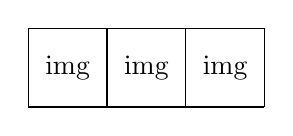
\begin{tikzpicture}
\draw (0,0) grid (3, 1);
\foreach \x in {1,...,3} {
	\node at (\x-0.5, 0.5) {img};
}
\end{tikzpicture}
\end{figure}

If the memory is arranged like this we can use some pointer maths ("dp[128*128*i]") to pass a pointer to the first pixel of each image to the fortran section.

\begin{code}
	int n_entry = tree->GetEntries();
	printf("Number of events: %d\n\n", n_entry);
	
	int j = 0;
	for (int i=0; (i<n_entry) && (i<l); i++) {
		tree->GetEntry(i);
		if (i % 100 == 0) {
			printf("%d\n", i);
		}
		if (N == 0) {
			continue;
		}
		a2img_orig(&N, x, y, z, sensor, &dp[128*128*j]);
// 		a2img(&N, x, y, z, &dp[128*128*j]);
// 		eta_beta(&pe, &px, &py, &pz, &eta[i], &beta[i]);
		j = j + 1;
	}
	return j;
}
\end{code}
\end{codeblock}

\printindex
\end{document}
